\documentclass{standalone}
\usepackage{tikz}
\usetikzlibrary{decorations.pathreplacing}
\usepackage{amsfonts}


\begin{document}
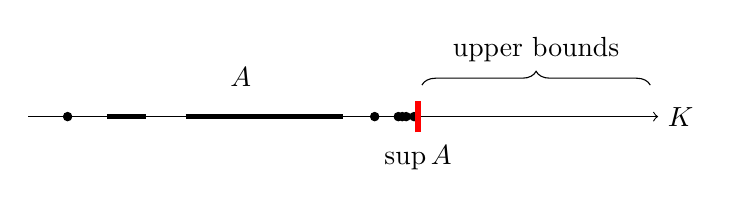
\begin{tikzpicture}
% Draw the real line
  \draw[->] (-4,0) -- (4,0) node[right] {$K$};
  
  % Draw the point 'x' and '0'
   
  \filldraw (-3.5,0) circle (1.5pt); 
 
  \draw[black, line width=2pt] (-3,0) -- (-2.5,0);
    \draw[black, line width=2pt] (-2,0) -- (0,0);

  \filldraw (0.4,0) circle (1.5pt);
  
  \filldraw (0.7,0) circle (1.5pt);
  \filldraw (0.75,0) circle (1.5pt);
  \filldraw (0.8,0) circle (1.5pt);
  \filldraw (0.9,0) circle (1.5pt);
  
  \node at (-1.3, 0.5) {$A$};
  
  % Draw the brace and label it
  \draw[decorate,decoration={brace,amplitude=5pt}] (1,0.4) -- (3.9,0.4) node[midway,above=5pt] {\mbox{upper bounds}};
  
   
  \draw[line width=2pt, red] (0.95,-0.2) -- (0.95,0.2);
  \node[anchor=south] at (0.95,-0.8) {$\sup A$};
  
  
  
  
  \end{tikzpicture}
\end{document}